\begin{figure}[t]
\centering
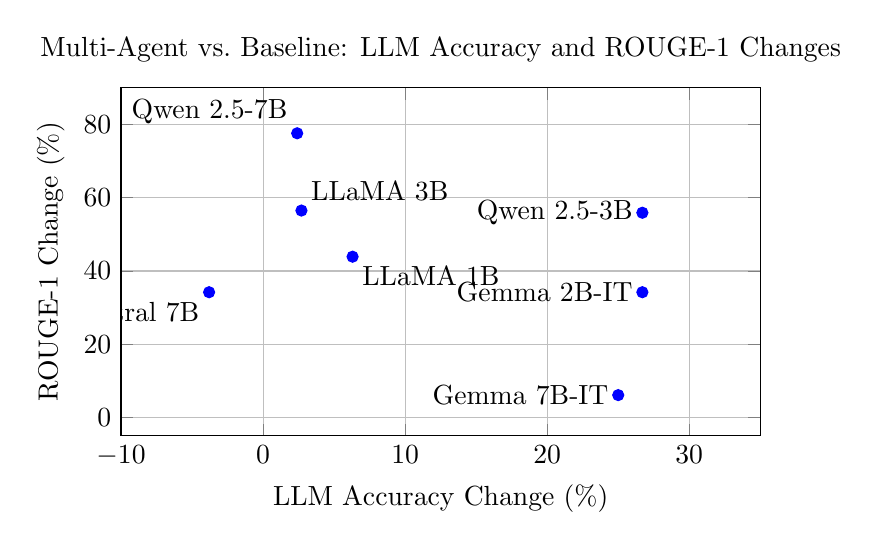
\begin{tikzpicture}
\begin{axis}[
    width=0.8\textwidth,
    height=6cm,
    xlabel={LLM Accuracy Change (\%)},
    ylabel={ROUGE-1 Change (\%)},
    xmin=-10, xmax=35,
    ymin=-5, ymax=90,
    grid=major,
    legend pos=south east,
    title={Multi-Agent vs.\ Baseline: LLM Accuracy and ROUGE-1 Changes}
]
% Data points
\addplot[only marks, mark=*, color=blue] coordinates {
    (6.3,  43.9)   % LLaMA 1B
    (2.4,  77.6)   % Qwen 2.5-7B
    (-3.8, 34.2)   % Mistral 7B
    (26.7, 55.9)   % Qwen 2.5-3B
    (26.7, 34.2)   % Gemma 2B-IT
    (25.0, 6.1)    % Gemma 7B-IT
    (2.7,  56.5)   % LLaMA 3B
};

% Labels
\node[above left]  at (axis cs:2.4,  77.6) {Qwen 2.5-7B};
\node[above right] at (axis cs:2.7,  56.5) {LLaMA 3B};
\node[below right] at (axis cs:6.3,  43.9) {LLaMA 1B};
\node[below left]  at (axis cs:-3.8, 34.2) {Mistral 7B};

\node[left] at (axis cs:26.7, 55.9) {Qwen 2.5-3B};
\node[left] at (axis cs:26.7, 34.2) {Gemma 2B-IT};
\node[left] at (axis cs:25.0, 6.1)  {Gemma 7B-IT};

\end{axis}
\end{tikzpicture}
\caption{Multi-agent vs.\ baseline changes in LLM accuracy and ROUGE-1 score across all
tested models (LLM accuracy from GPT-4.1 judge). The decoupling of these two metrics---high ROUGE-1 gains do not imply high accuracy gains, and vice versa---is itself a finding, indicating that lexical overlap and LLM-judged accuracy capture distinct aspects of answer quality.}
\label{fig:tradeoff}
\end{figure}
